\section{Experimentacìon y pruebas}
En este capítulo se llevan a cabo pruebas a los módulos desarrollados con el objetivo de realizar un estudio que permita identificar áreas de mejora y optimizar su funcionamiento futuro.
\subsection{Pruebas funcionales}
Mediante el uso de Selenium, una herramienta automatizada para realizar pruebas funcionales en aplicaciones web, se evaluaron las diferentes partes de los módulos, tanto de forma individual como conjunta. Esto permitió verificar su correcto funcionamiento y detectar posibles errores o áreas de mejora en la interacción del usuario con cada módulo.
En cada uno de los casos, se verificó el funcionamiento de todos los botones disponibles, tanto los botones físicos como aquellos ubicados en la interfaz. Se realizaron pruebas exhaustivas para asegurar que cada botón respondiera correctamente y ejecutará las acciones esperadas, garantizando una interacción fluida y sin errores en el uso de los módulos.A continuación, se presentan los resultados e instrucciones obtenidas en las pruebas conjuntas. Para la revisión de las pruebas individuales, ir a la sección de anexos.

\subsubsection{Pruebas conjuntas}

\begin{figure}[ht]
  \centering
  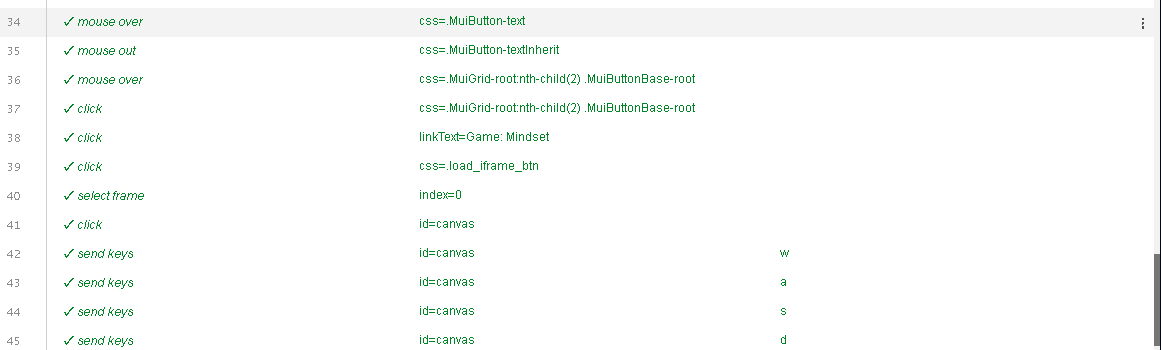
\includegraphics[width=1\linewidth]{Imagenes/Imagen11.png}
  \caption{Imagen de referencia sobre instrucciones de gamificación para los módulos conjuntos, Elaboración propia}
  \label{fig:imagen1pruebas}
\end{figure}
\begin{figure}[ht]
  \centering
  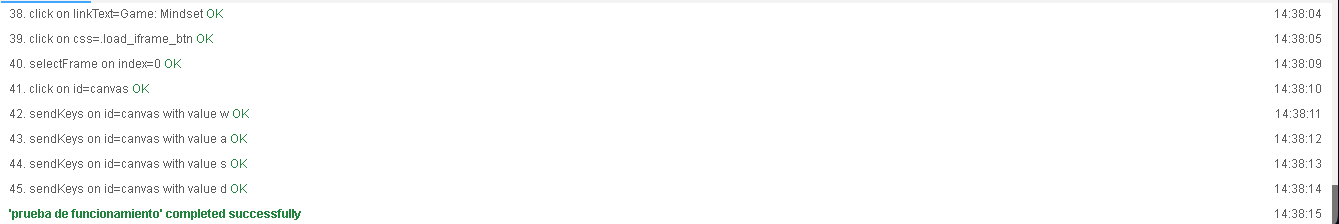
\includegraphics[width=1\linewidth]{Imagenes/Imagen12.png}
  \caption{Imagen de referencia sobre resultados de gamificación para los módulos conjuntos, Elaboración propia}
  \label{fig:imagen2pruebas}
\end{figure}

\subsection{Pruebas de usabilidad en voz alta}

Se realizaron tres pruebas de usabilidad en voz alta, las cuales consisten en pedir a los usuarios que verbalicen sus pensamientos mientras interactúan con un software. A continuación, se presenta un breve resumen de lo observado en cada una.

\subsubsection{Prueba 1}
La primera prueba tuvo una duración de 36 minutos. Esta comenzó con el módulo fitness, específicamente con la sección para la corrección de la mala postura, la cual transcurrió con normalidad. El usuario se mostró animado durante esta etapa.
Se continuó con la segunda sección del mismo módulo, que también transcurrió sin dificultades. El usuario mantuvo una actitud tranquila a lo largo de esta parte.
\\\\
Posteriormente, se pasó al módulo mindset, donde se realizaron los dos primeros niveles sin inconvenientes. El usuario se mostró animado durante estas actividades.
\\\\
Al llegar al tercer nivel, presentó algunas dificultades con el movimiento del personaje. Sin embargo, continuó al cuarto nivel, donde, tras un breve periodo de observación, completó el nivel rápidamente. Finalmente, en el último nivel, el usuario solicitó asistencia para completarlo, lo que evidencia un grado de dificultad probablemente demasiado elevado.

\subsubsection{Prueba 2}

La segunda prueba tuvo una duración de 1 hora y 38 minutos. Comenzó con la gamificación sobre el mindset,
 la cual no presentó mayores impedimentos para completar el nivel 1 de manera rápida.
  Sin embargo, el segundo nivel requirió un tiempo considerable, aproximadamente 35 minutos, 
  donde se observó un entendimiento de la utilidad de la balanza, aunque surgieron problemas 
  para identificar el orden correcto en el que se debían colocar los bloques.
\\\\
El tercer nivel se completó de forma normal y no presentó grandes dificultades.
 En el cuarto nivel, aunque inicialmente hubo un poco de dificultad para comprender las mecánicas,
  se logró superar de forma rápida tras entenderlas. Finalmente, el último nivel tomó alrededor
   de 25 minutos en completarse. Durante este nivel, el usuario presentó dificultades significativas
    y tuvo que solicitar asistencia, lo que indica que la dificultad podría ser demasiado elevada.
  \\  \\
    Posteriormente, se continuó con la sección para la corrección de la mala postura en el módulo fitness, la cual no presentó dificultad alguna y prosiguió con normalidad. Sin embargo, es importante destacar que, después de un tiempo, el usuario parecía aburrirse debido a la baja velocidad del desarrollo una vez que se acostumbró a la dinámica del ejercicio.
\\\\
Finalmente, se pasó a la sección destinada a los ejercicios para ayudar con el túnel carpiano en el módulo fitness. En esta parte, no se presentaron mayores dificultades, salvo por los primeros momentos, donde el usuario tuvo problemas para comprender los controles del ejercicio.

\subsubsection{Prueba 3}
La tercera prueba tuvo una duración de 34 minutos.
La prueba comenzó con la sección de corrección de la postura del módulo fitness, la cual se completó sin ninguna dificultad. El usuario se mostró animado durante esta parte.
\\\\
Posteriormente, inició la segunda sección del mismo módulo, enfocada en ejercicios para ayudar con el túnel carpiano. Aunque presentó una leve dificultad para comprender las instrucciones al inicio, pudo continuar sin complicaciones tras unos momentos.
\\\\
A continuación, el usuario pasó al módulo mindset. Completó el primer nivel sin dificultades y logró superar el segundo nivel por mera casualidad, sin necesidad de utilizar la balanza.
En el tercer nivel, comprendió rápidamente la mecánica, y aunque necesitó varios intentos, logró completarlo con éxito. El cuarto nivel lo superó a base de repetición e intentos, hasta que comprendió las pistas necesarias para avanzar.
\\\\
Finalmente, en el último nivel, el usuario lo completó basándose en su memoria y repeticiones previas, sin necesitar de las pistas proporcionadas en el juego.